\documentclass[./../../paper.tex]{subfiles}
\graphicspath{{\subfix{./../../figures/}}}

\begin{document}


\autoref{fig:exp5-winner} displays the results of running each algorithm on a set of different datasets. The figure shows clear dominance of the evolutionary model all the models across all datasets. 

\begin{figure}[htbp]
    \centering
    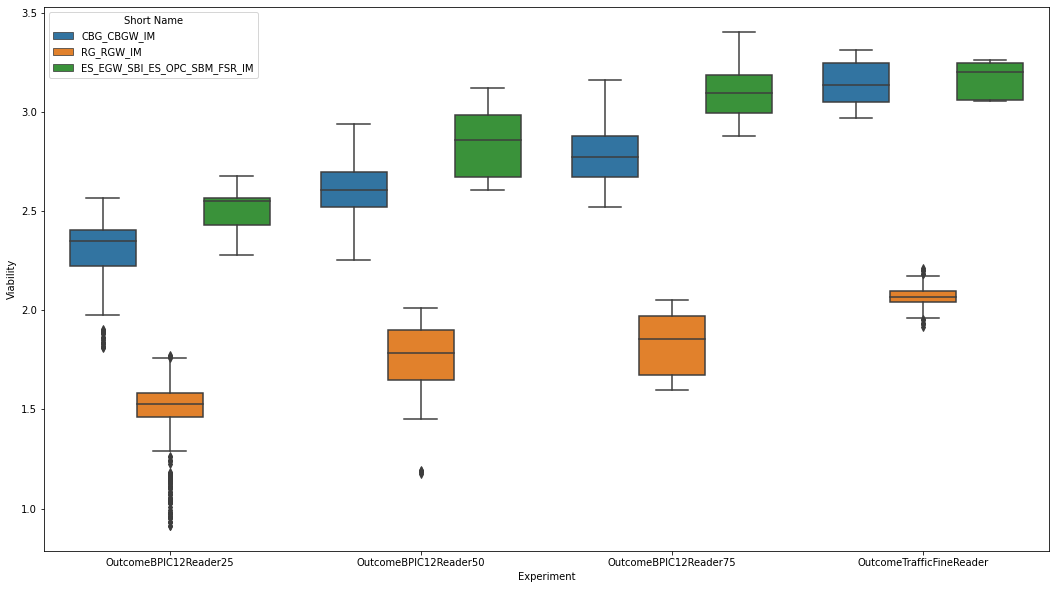
\includegraphics[width=\textwidth]{figures/generated/exp5_winner_overall.png}
    \caption{Boxplots of the viability of each models' generated counterfactuals across a herterogeneous collection of datasets.}
    \label{fig:exp5-winner}
\end{figure}

Here, \emph{CBI-ES-UC3-SBM-RR} and \emph{CBI-RWS-OPC-SBM-FSR} display a higher median of viability across all datasets. 
This is unsurprising as the evolutionary algorithm use inititiators that are based on the baselines. 
However, it is surprising that the evolutionary models consistently outperform the \ModelCBG (green) across all datasets. In 6 out of 9 datasets we see an improvement of at least 0.15. 
From \autoref{app:exp5-winner-datasets} we see that the gap often occurs because of much higher similarity and sparsity scores. The highest median is reached for \emph{CBI-RWS-OPC-SBM-FSR} at 2.94. 
The \ModelRNG never manages to come even close to the case based model. Except for the BPIC12-100 dataset, the \ModelRNG has a median below 2. 


\begin{table}
    \centering    
    \resizebox{\linewidth}{!}{
    \begin{tabular}{lllllllllll}
\toprule
\multicolumn{4}{l}{Factual Seq.} & \multicolumn{4}{l}{Our CF Seq.} & \multicolumn{3}{l}{DiCE4EL CF Seq.} \\
Amount & Activity & Outcome & Resource & Amount & Activity & Outcome & Resource & Activity & Resource & Amount \\
\midrule
150 & A-SUBMITTED & 0 & 112 &  &  &  &  &  &  &  \\
150 & A-PARTLYSUBMITTED & 0 & 112 &  &  &  &  &  &  &  \\
150 & A-PREACCEPTED & 0 & 112 &  &  &  &  &  &  &  \\
150 & W-Completeren aanvraag & 0 & 112 &  &  &  &  &  &  &  \\
150 & W-Completeren aanvraag & 0 & 111 &  &  &  &  &  &  &  \\
150 & W-Completeren aanvraag & 0 & 889 &  &  &  &  &  &  &  \\
150 & W-Completeren aanvraag & 0 & 889 &  &  &  &  &  &  &  \\
150 & W-Completeren aanvraag & 0 & 9 &  &  &  &  &  &  &  \\
150 & A-ACCEPTED & 0 & 9 &  &  &  &  &  &  &  \\
150 & A-FINALIZED & 0 & 9 & 150 & A-SUBMITTED & 1 & 112 &  &  &  \\
150 & O-SELECTED & 0 & 9 & 150 & A-PARTLYSUBMITTED & 1 & 112 &  &  &  \\
150 & O-CREATED & 0 & 9 & 150 & A-PREACCEPTED & 1 & 112 & A-SUBMITTED & 112 & 150 \\
150 & O-SENT & 0 & 9 & 150 & W-Completeren aanvraag & 1 & 111 & A-PARTLYSUBMITTED & 112 & 150 \\
150 & W-Completeren aanvraag & 0 & 9 & 150 & W-Completeren aanvraag & 1 & 111 & A-PREACCEPTED & 112 & 150 \\
150 & W-Nabellen offertes & 0 & 9 & 150 & A-ACCEPTED & 1 & 111 & A-ACCEPTED & 1 & 150 \\
150 & W-Nabellen offertes & 0 & 9 & 150 & A-FINALIZED & 1 & 111 & O-SELECTED & 1 & 150 \\
150 & O-SENT-BACK & 0 & 129 & 150 & O-SELECTED & 1 & 111 & A-FINALIZED & 1 & 150 \\
150 & W-Nabellen offertes & 0 & 129 & 150 & O-CREATED & 1 & 111 & O-CREATED & 1 & 150 \\
150 & W-Valideren aanvraag & 0 & 138 & 150 & O-SENT & 1 & 111 & O-SENT & 1 & 150 \\
150 & O-DECLINED & 0 & 138 & 150 & W-Completeren aanvraag & 1 & 111 & W-Completeren aanvraag & 1 & 150 \\
150 & A-DECLINED & 0 & 138 & 150 & O-SENT-BACK & 1 & 149 & O-SENT-BACK & 11259 & 150 \\
150 & W-Valideren aanvraag & 0 & 138 & 150 & W-Nabellen offertes & 1 & 149 & W-Nabellen offertes & 11259 & 150 \\
 &  &  &  & 150 & O-ACCEPTED & 1 & 629 & O-ACCEPTED & 9 & 150 \\
\bottomrule
\end{tabular}
}
    \caption{A comparison between the \ModelCBG and D4EL}
    \label{tbl:cf-cbg}
\end{table}
\begin{table}
    \centering    
    \resizebox{\linewidth}{!}{
        \begin{tabular}{lllllllllll}
\toprule
\multicolumn{4}{l}{Factual Seq.} & \multicolumn{4}{l}{Our CF Seq.} & \multicolumn{3}{l}{DiCE4EL CF Seq.} \\
Amount & Activity & Outcome & Resource & Amount & Activity & Outcome & Resource & Activity & Resource & Amount \\
\midrule
150 & A-SUBMITTED & 0 & 112 &  &  &  &  &  &  &  \\
150 & A-PARTLYSUBMITTED & 0 & 112 &  &  &  &  &  &  &  \\
150 & A-PREACCEPTED & 0 & 112 &  &  &  &  &  &  &  \\
150 & W-Completeren aanvraag & 0 & 112 &  &  &  &  &  &  &  \\
150 & W-Completeren aanvraag & 0 & 111 &  &  &  &  &  &  &  \\
150 & W-Completeren aanvraag & 0 & 889 &  &  &  &  &  &  &  \\
150 & W-Completeren aanvraag & 0 & 889 &  &  &  &  &  &  &  \\
150 & W-Completeren aanvraag & 0 & 9 &  &  &  &  &  &  &  \\
150 & A-ACCEPTED & 0 & 9 & 1 & A-SUBMITTED & 1 & 112 &  &  &  \\
150 & A-FINALIZED & 0 & 9 & 1 & A-PARTLYSUBMITTED & 1 & 112 &  &  &  \\
150 & O-SELECTED & 0 & 9 & 1 & A-PREACCEPTED & 1 & 112 &  &  &  \\
150 & O-CREATED & 0 & 9 & 1 & A-ACCEPTED & 1 & 861 & A-SUBMITTED & 112 & 150 \\
150 & O-SENT & 0 & 9 & 1 & A-FINALIZED & 1 & 861 & A-PARTLYSUBMITTED & 112 & 150 \\
150 & W-Completeren aanvraag & 0 & 9 & 1 & O-SELECTED & 1 & 861 & A-PREACCEPTED & 112 & 150 \\
150 & W-Nabellen offertes & 0 & 9 & 1 & O-CREATED & 1 & 861 & A-ACCEPTED & 1 & 150 \\
150 & W-Nabellen offertes & 0 & 9 & 1 & O-SENT & 1 & 861 & O-SELECTED & 1 & 150 \\
150 & O-SENT-BACK & 0 & 129 & 1 & W-Completeren aanvraag & 1 & 861 & A-FINALIZED & 1 & 150 \\
150 & W-Nabellen offertes & 0 & 129 &  & W-Nabellen offertes & 1 & 11189 & O-CREATED & 1 & 150 \\
150 & W-Valideren aanvraag & 0 & 138 & 159 & W-Nabellen offertes & 1 & 861 & O-SENT & 1 & 150 \\
150 & O-DECLINED & 0 & 138 & 1 & O-SENT-BACK & 1 & 129 & W-Completeren aanvraag & 1 & 150 \\
150 & A-DECLINED & 0 & 138 & 15363 & W-Nabellen offertes & 1 & 912 & O-SENT-BACK & 11259 & 150 \\
150 & W-Valideren aanvraag & 0 & 138 & 14536 & W-Valideren aanvraag & 1 & 129 & W-Nabellen offertes & 11259 & 150 \\
 &  &  &  & 1 & O-ACCEPTED & 1 & 138 & O-ACCEPTED & 9 & 150 \\
\bottomrule
\end{tabular}
}
        \caption{A comparison between the CBI-ES-UC3-SBM-RR and D4EL}
        \label{tbl:cf-rr}
\end{table}
\begin{table}
    \centering    
    \resizebox{\linewidth}{!}{
    \begin{tabular}{lllllllllll}
\toprule
\multicolumn{4}{l}{Factual Seq.} & \multicolumn{4}{l}{Our CF Seq.} & \multicolumn{3}{l}{DiCE4EL CF Seq.} \\
Amount & Activity & Outcome & Resource & Amount & Activity & Outcome & Resource & Activity & Resource & Amount \\
\midrule
150 & A-SUBMITTED & 0 & 112 &  &  &  &  &  &  &  \\
150 & A-PARTLYSUBMITTED & 0 & 112 &  &  &  &  &  &  &  \\
150 & A-PREACCEPTED & 0 & 112 &  &  &  &  &  &  &  \\
150 & W-Completeren aanvraag & 0 & 112 &  & A-SUBMITTED & 1 & 112 &  &  &  \\
150 & W-Completeren aanvraag & 0 & 111 &  & A-PARTLYSUBMITTED & 1 & 112 &  &  &  \\
150 & W-Completeren aanvraag & 0 & 889 &  & A-PREACCEPTED & 1 & 112 &  &  &  \\
150 & W-Completeren aanvraag & 0 & 889 &  & W-Completeren aanvraag & 1 & 861 &  &  &  \\
150 & W-Completeren aanvraag & 0 & 9 & 70 & W-Completeren aanvraag & 1 & 861 &  &  &  \\
150 & A-ACCEPTED & 0 & 9 & 70 & W-Completeren aanvraag & 1 & 861 &  &  &  \\
150 & A-FINALIZED & 0 & 9 & 70 & A-ACCEPTED & 1 & 861 &  &  &  \\
150 & O-SELECTED & 0 & 9 & 70 & A-FINALIZED & 1 & 861 &  &  &  \\
150 & O-CREATED & 0 & 9 & 70 & O-SELECTED & 1 & 861 & A-SUBMITTED & 112 & 150 \\
150 & O-SENT & 0 & 9 & 70 & O-CREATED & 1 & 861 & A-PARTLYSUBMITTED & 112 & 150 \\
150 & W-Completeren aanvraag & 0 & 9 & 70 & O-SENT & 1 & 861 & A-PREACCEPTED & 112 & 150 \\
150 & W-Nabellen offertes & 0 & 9 & 70 & W-Completeren aanvraag & 1 & 861 & A-ACCEPTED & 1 & 150 \\
150 & W-Nabellen offertes & 0 & 9 & 70 & W-Nabellen offertes & 1 & 109 & O-SELECTED & 1 & 150 \\
150 & O-SENT-BACK & 0 & 129 & 70 & W-Nabellen offertes & 1 & 861 & A-FINALIZED & 1 & 150 \\
150 & W-Nabellen offertes & 0 & 129 &  &  &  &  & O-CREATED & 1 & 150 \\
150 & W-Valideren aanvraag & 0 & 138 & 70 & O-SENT-BACK & 1 & 789 & O-SENT & 1 & 150 \\
150 & O-DECLINED & 0 & 138 & 70 & W-Nabellen offertes & 1 & 789 & W-Completeren aanvraag & 1 & 150 \\
150 & A-DECLINED & 0 & 138 &  &  &  &  & O-SENT-BACK & 11259 & 150 \\
150 & W-Valideren aanvraag & 0 & 138 &  & W-Valideren aanvraag & 1 & 138 & W-Nabellen offertes & 11259 & 150 \\
 &  &  &  & 70 & O-ACCEPTED & 1 & 11289 & O-ACCEPTED & 9 & 150 \\
\bottomrule
\end{tabular}
}
    \caption{A comparison between the CBI-RWS-OPC-SBM-FSR and D4EL}
    \label{tbl:cf-fsr}
\end{table}
\begin{table}
    \centering    
    \resizebox{\linewidth}{!}{
    \begin{tabular}{lllllllllll}
\toprule
\multicolumn{4}{l}{Factual Seq.} & \multicolumn{4}{l}{Our CF Seq.} & \multicolumn{3}{l}{DiCE4EL CF Seq.} \\
Amount & Activity & Outcome & Resource & Amount & Activity & Outcome & Resource & Activity & Resource & Amount \\
\midrule
 &  &  &  & 11 247 & A-PARTLYSUBMITTED & 1 &  &  &  &  \\
 &  &  &  & 10 159 & A-FINALIZED & 1 &  &  &  &  \\
 &  &  &  & 13 939 & O-SENT & 1 &  &  &  &  \\
15 500 & A-SUBMITTED & 0 & 112 & 10 550 & A-APPROVED & 1 &  &  &  &  \\
15 500 & A-PARTLYSUBMITTED & 0 & 112 & 25 608 & A-APPROVED & 1 &  &  &  &  \\
15 500 & A-PREACCEPTED & 0 & 112 & 29 560 & W-Nabellen offertes & 1 &  &  &  &  \\
15 500 & W-Completeren aanvraag & 0 & 112 & 4 665 & O-CANCELLED & 1 &  &  &  &  \\
15 500 & W-Completeren aanvraag & 0 & 111 & 19 918 & O-SELECTED & 1 &  &  &  &  \\
15 500 & W-Completeren aanvraag & 0 & 889 & 16 922 & W-Completeren aanvraag & 1 &  &  &  &  \\
15 500 & W-Completeren aanvraag & 0 & 889 &  &  &  &  &  &  &  \\
15 500 & W-Completeren aanvraag & 0 & 9 & 19 969 & A-SUBMITTED & 1 &  &  &  &  \\
15 500 & A-ACCEPTED & 0 & 9 & 13 066 & A-PREACCEPTED & 1 &  &  &  &  \\
15 500 & A-FINALIZED & 0 & 9 &  &  &  &  &  &  &  \\
15 500 & O-SELECTED & 0 & 9 & 25 535 & A-DECLINED & 1 &  &  &  &  \\
15 500 & O-CREATED & 0 & 9 &  &  &  &  & A-SUBMITTED & 112 & 15 500 \\
15 500 & O-SENT & 0 & 9 & 21 437 & O-CREATED & 1 &  & A-PARTLYSUBMITTED & 112 & 15 500 \\
15 500 & W-Completeren aanvraag & 0 & 9 & 17 469 & W-Beoordelen fraude & 1 &  & A-PREACCEPTED & 112 & 15 500 \\
15 500 & W-Nabellen offertes & 0 & 9 &  &  &  &  & A-ACCEPTED & 1 & 15 500 \\
15 500 & W-Nabellen offertes & 0 & 9 & 29 395 & W-Completeren aanvraag & 1 &  & O-SELECTED & 1 & 15 500 \\
15 500 & O-SENT-BACK & 0 & 129 & 9 053 & O-SENT-BACK & 1 &  & A-FINALIZED & 1 & 15 500 \\
15 500 & W-Nabellen offertes & 0 & 129 &  &  &  &  & O-CREATED & 1 & 15 500 \\
15 500 & W-Valideren aanvraag & 0 & 138 & 11 627 & A-FINALIZED & 1 &  & O-SENT & 1 & 15 500 \\
15 500 & O-DECLINED & 0 & 138 & 41 470 & W-Valideren aanvraag & 1 &  & W-Completeren aanvraag & 1 & 15 500 \\
15 500 & A-DECLINED & 0 & 138 & 16 381 & O-SENT-BACK & 1 &  & O-SENT-BACK & 11259 & 15 500 \\
15 500 & W-Valideren aanvraag & 0 & 138 & 2 828 & A-ACCEPTED & 1 &  & W-Nabellen offertes & 11259 & 15 500 \\
 &  &  &  & 8 834 & O-ACCEPTED & 1 &  & O-ACCEPTED & 9 & 15 500 \\
\bottomrule
\end{tabular}
}
    \caption{A comparison between the \ModelRNG and D4EL}
    \label{tbl:cf-rng}
\end{table}

In tables \ref{tbl:cf-cbg}, \ref{tbl:cf-rr}, \ref{tbl:cf-fsr} and \ref{tbl:cf-rng} we show generations of all models and compare them to DiCE4EL. We see that all models return reasonable counterfactuals, except the \ModelRNG. This model does not seem to follow any pattern.  


% TODO
% A notable observation occurs in the processing time. Although all models require more time to produce their results, if we increase the maximum length of sequences, the evolutionary algorithms require substiantially more time. \autoref{tbl:exp5_duration} shows, the processing time is much higher than the baseline models. On average, \attention{evo model} require \attention{duration in seconds}, while \attention{other models} require \attention{XX}, \attention{XX} and \attention{XX}, respectively.


\end{document}